\chapter{Continuum Mechanics and Finite Element Method} \label{ch:continuum_mechanics}

This chapter deals with the concepts needed to described the behavior of a solid undergoing large deformation, as well as, the conservation principles that ensure its mechanical equilibrium.
It also presents a succint overview of the Finite Element Method as a tool to solve mechanical initial value equilibrium problem.
These topics are broadly covered in the literature and here the approach used follows \cite{de_souza_neto_computational_2008},

\section{Kinematics of Deformation}

\subsection{Motion}

Let a deformable body $\mathscr{B}$ occupy an open region $\Omega_0$ of the tridimensional Euclidean space $\mathscr{E}$ with a regular boundary $\partial \Omega_0$ in its reference configuration.
Its motion, depicted in Figure \ref{}, is defined by a smooth one-to-one function
\begin{equation}
    \vect \varphi\colon \Omega\times \mathscr{R}\to \mathscr{E},
\end{equation}
mapping each material particle of coordinates $\vect X$ in the reference configuration to its position $\vect x$ in the deformed configuration, for a given instant of time $t$, as
\begin{highlight}
    \begin{equation}
        \vect x = \vect \varphi(\vect X, t)=\bm \varphi_t(\bm X).
    \end{equation}
\end{highlight}

\enlargethispage{\baselineskip}
Thus, the displacement field is defined as
\begin{equation}
    \vect u(\vect X, t) = \vect \varphi(\vect X, t) - \vect X,
\end{equation}
and, since the function that defines the motion is one-to-one, the reference configuration can be recovered as
\begin{equation}
    \vect X = \vect \varphi^{-1} (\vect x, t) = \vect x - \vect u(\vect \varphi^{-1}(\vect x, t),t),
\end{equation}
where $\vect \varphi^{-1}$ is the reference mapping function.

\begin{figure}
  \centering
  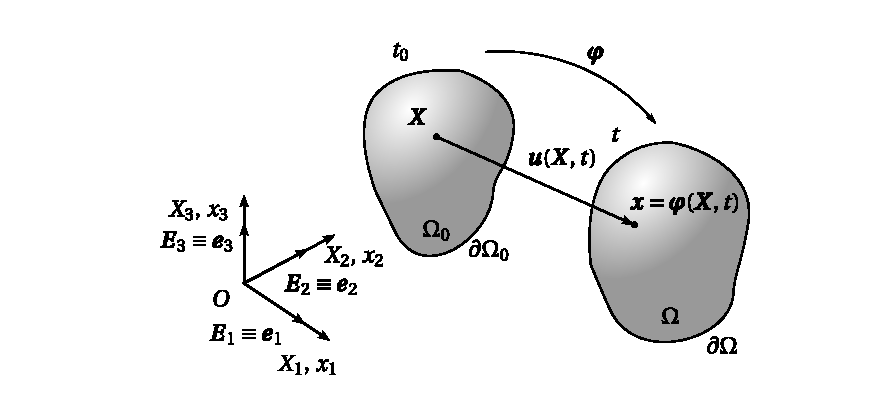
\includegraphics[width=.9\textwidth]{motion}
  \caption{Motion}
\label{fig:motion}
\end{figure}

\subsection{Material and spatial descriptions}

Dealing with finite deformations, the behavior of the body under analysis can be described with respect to the reference configuration, using the so-called material or Lagrangian description, or to the deformed configuration, using the so-called spatial or Eulerian description.

In the Lagrangian description any field, be it scalar, vectorial or tensorial defined over the body is expressed as a function of the reference configuration, $\vect X \in \Omega_0$.
On the other hand, the Eulerian descritpion of same field is done using the deformed configuration, $\vect x\in \Omega$.

As such let $\alpha(\vect x,t)$ be a spatial field and $\beta(\vect X, t)$ a material field.
Their material $\alpha_m$ and spatial $\beta_s$ desctiptions are given by
\begin{align}
    \alpha_m(\vect X, t) &=\alpha(\vect \varphi(\vect X, t),t),\\
    \beta_s(\vect x, t) &= \beta(\vect \varphi^{-1}(\vect x, t),t),
\end{align}
noting that any field associated with a motion of $\mathscr{B}$ can be expressed as a function of time and the point's position in the reference or deformed configuration.

The same distinction between material and spatial descriptions applies to operators such as the divergence and the gradient.
The spatial and material gradients, $\nabla$ and $\nabla_0$, respectively, are defined as
\begin{equation}
    \nabla \alpha = \frac{\partial}{\partial \vect x}\alpha(\vect x,t),\quad
    \nabla_0 \beta = \frac{\partial}{\partial \vect X}\beta (\vect X, t),
\end{equation}
where the derivatives are taken with respect to the spatial and reference configuration accordingly.

% \subsection{Velocity and acceleration}
%
% For solid dynamical problems, both the velocity and the acceleration corresponding to the motion \(\bm \varphi\) must be considered.
% The velocity is defined as
% \begin{gather}
%   \bm V = \frac{\partial \bm \varphi}{\partial t},\\
%   \bm v_t = \bm V_t \circ \bm \varphi_t^{-1},
% \end{gather}
% in the material and and spatial descriptions, respectively.
% See Figure~\ref{}.
% The formulas for the acceleration, again in both material and spatial descriptions, are
% \begin{gather}
%  \bm A = \frac{\partial \bm V}{\partial t},\\
%  \bm a = \bm A_t\circ \bm \varphi^{-1}_t.
% \end{gather}
% The spatial acceleration \(\bm a\) is related to the spatial velocity \(\bm v\) by
% \begin{equation}
%   \bm a = \dot{\bm v} = \frac{\partial \bm v}{\partial t} + \nabla \bm v\cdot \bm v.
% \end{equation}


\subsection{Deformation gradient}

The deformation gradient, a second order tensor denoted by $\mat F$, is defined as
\begin{highlight}
    \begin{equation}
            \mat F(\vect X,t)\equiv \nabla_0\vect\varphi(\vect X,t) =\frac{\partial \vect x}{\partial \vect X},
    \end{equation}
\end{highlight}
or, taking into account that
\begin{equation}
    \vect x = \vect X + \vect u(\vect X, t),
\end{equation}
it can be expressed as
\begin{equation}
    \mat F(\vect X, t) = \mat I + \nabla_0 \bm u.
\end{equation}

The deformation gradient relates the relative position between two neighboring material particles before and after deformation.
To see this let $\vect X$ be the coordinates of some material particle in the reference configuration and $\vect X + d\vect X$ the coordinates of some material particle in its neighborhood, their corresponding coordinates in the deformed configuration are given by
\begin{gather}
    \vect X = \vect x - \vect u(\vect X, t), \label{eq:mat_pos}\\
    \vect X + d\vect X = \vect x + d\vect x -\vect u(\vect X +d\vect X, t). \label{eq:mat_pos_delta}
\end{gather}
Subtracting Equation \eqref{eq:mat_pos} to Equation \eqref{eq:mat_pos_delta}, it is found that
\begin{align}
    d\vect X &= d\vect x +\vect u(\vect X, t)-\vect u(\vect X +d\vect X, t)\\
             &=(\mat I +\nabla_0 \vect u(\vect X, t))\; d\vect x\\
             &=\mat F\;d\vect x.
\end{align}

Due to this relation, it can be shown that the determinat of the deformation gradient has a physical meaning.
It is the local unit volume change, that is,
\begin{highlight}
\begin{equation}
   J\equiv \text{det}\;\mat F = \frac{dv}{dv_0}, \label{eq:det_grad_func}
\end{equation}
\end{highlight}
where $dv_0$ is an infinitesimal volume of the body in its reference configuration and $dv$ the infinitesimal volume after deformation.

\subsubsection{Isochoric/Volumetric decomposition}

Any deformation can be locally decomposed in volumetric and isochoric (or distortional) components.
From Equation \eqref{eq:det_grad_func} it can be gathered that an isochoric deformation is characterized by $J=1$.
As such, the deformation gradient can be decomposed as
\begin{equation}
    \mat F = \mat F_\text{iso} \mat F_\text{vol} = \mat F_\text{vol} \mat F_\text{iso},
\end{equation}
where the isochoric and columetric components are defined by
\begin{equation}
    \mat F_\text{iso} = (\text{det}\;\mat F)^{-\frac{1}{3}},\quad \mat F_\text{vol} = (\text{det}\;\mat F)^{\frac{1}{3}}\mat I.
\end{equation}

\subsubsection{Polar decomposition}

The deformation gradient can also be decomposed in rotation and stretch components, the so-called polar decomposition, defined as
\begin{highlight}
    \begin{equation}
        \mat F = \mat R\mat U = \mat V\mat R, \label{eq:polar_decomposition}
    \end{equation}
\end{highlight}
where $\mat R$ is the proper orthogonal rotation tensor and $\mat U$ and $\mat V$ are the symmetric positive right and left stretch tensors, respectively.

Equation \eqref{eq:polar_decomposition} has a physical interpretation with the right polar decomposition ($\mat F= \mat R\mat U$) corresponding to a stretch mapping followed by a rotation, and the left polar decomposition ($\mat F = \mat V\mat R$) corresponding to a rotation followed by a stretch mapping.
\
The right $\mat U$ and left $\mat V$ stretch tensors are related through the rotation matrix $\mat R$ as
\begin{equation}
    \mat V = \mat R\mat U\mat R^T,
\end{equation}
and can be obtained from deformation gradient by
\begin{highlight}
    \begin{equation}
        \mat C \equiv \mat U^2 = \mat F^T \mat F,\quad \mat B \equiv \mat V^2 = \mat F\mat F^T.,
    \end{equation}
\end{highlight}
where $\mat C$ and $\mat B$ are the right and left Cauchy-Green strain tensors.

Since $\mat U$ and $\mat V$ are symmetric tensors, they admit the spectral decomposition
\begin{equation}
    \mat U = \sum_{i=1}^3 \lambda_i \vect E_i^* \otimes \vect E_i^*,\quad \mat V = \sum_{i=1}^3 \lambda_i \vect e_i^*\otimes \vect e_i^*,
\end{equation}
where $\lambda_i$, $i=1,2,3,$ are the eigenvalues of both $\mat U$ and $\mat V$ and $\vect E_i^*$ and $\vect e_i^*$ are the respective eigenvectors.

The eigenvectors of left $\mat V$ and right $\mat U$ stretch tensors are related through
\begin{equation}
    \vect e_i^*= \mat R \vect E_i^*.
\end{equation}
forming two orthogonal bases.
These vectors define the Lagrangian and Eulerian principal directions, respectively, allowing for the expression of the local stretching from a material particle, associated with any deformation, as a superposition of stretches along the three mutual orthogonal directions.,

% \textcolor{red}{
% For solid dynamical problems, material time differentiation of the deformation and the strain measures need to be introduced. The first and second derivative of the displacement field \(u(X, t)\). li.e. the material velocity and acceleration, \(\dot{u}\) and \(\ddot{u}\), respectively, result in)
% where \((2.2)\) can be used to show that due to the constant initial position \(X\) )
% \[
% \hat{\boldsymbol{x}}(\boldsymbol{X}, t) \equiv \overline{\boldsymbol{u}}(\boldsymbol{X}, t)
% \]
% According to \((2.3)\), the material velocity gradient results in
% With the material gradient operator \(\operatorname{Grad}(\cdot)\). Equation \((2.23)\) can be reformulated, yielding the Ispatial velocity gradient
% and its symmetric part
% \[
% \begin{array}{c}
% \boldsymbol{L}=\dot{\boldsymbol{F}} \cdot \boldsymbol{F}^{-1} \\
% \boldsymbol{D}=\frac{1}{2}\left(\boldsymbol{L}+\boldsymbol{L}^{\top}\right)
% \end{array}
% \]
% The rate of the Green-Lagrange strain tensor results in the material strain rate tensor
% \[
% \dot{E}_{\mathrm{GL}}=\frac{1}{2} \dot{C}=\boldsymbol{F}^{\mathrm{T}} \cdot \boldsymbol{D} \cdot \boldsymbol{F}
% \]
% which can be expressed as pull-back of the symmetric spatial strain rate tensor \(D\). Via the Liederivative or Oldroyd-Lie derivative of the Euler-Almansi strain tensor \(\mathcal{L}_{t}\left[\boldsymbol{E}_{\mathrm{EA}}\right]\), which represents an objective material time derivative, a relation to the rate of the Euler-Almansi strain tensor is achieved as
% \[
% \mathcal{L}_{t}\left[\boldsymbol{E}_{\mathrm{EA}}\right]=\varphi\left[\frac{\mathrm{d}}{\mathrm{d} t}\left(\varphi^{-1}\left[\boldsymbol{E}_{\mathrm{EA}}\right]\right)\right]=\boldsymbol{D}=\boldsymbol{F}^{-\top} \cdot \dot{\boldsymbol{E}}_{\mathrm{GL}} \cdot \boldsymbol{F}^{-1}
% \]
% Moreover, the rate of volume changes is described by \(\dot{J}\) and can be expressed through
% \[
% \dot{J}=J \operatorname{tr} \boldsymbol{D}
% \]}


\section{Strain tensors}

In Continuum Mechanics there are two main families of strain tensors derived from the deformation gradient and used to describe the body deformation.
The Lagrange family strain tensors are defined as
\begin{equation}
    \mat E^{(m)} =\begin{cases} \displaystyle{\frac{1}{m} (\mat U^m - \mat I)},&\quad m\neq 0,\\[12pt] \ln(\mat U),& \quad m=0, \end{cases}
\end{equation} where $m$ is a real number, and likewise, the Euler family strain tensors are defined as
\begin{equation}
     \mat \varepsilon^{(m)} =\begin{cases} \displaystyle{\frac{1}{m} (\mat V^m - \mat I)},&\quad m\neq 0,\\[12pt] \ln(\mat V),& \quad m=0, \end{cases}
\end{equation}
where $m$ is also real number.

\enlargethispage{\baselineskip}
In particular, choosing $m=0$, one obtains the so-called material and spatial logarithmic strain tensors
\begin{highlight}[innertopmargin=-5pt]
    \begin{align}
        \mat E^{(0)} &\equiv \ln[\mat U] = \sum_{i=1}^3 \ln \lambda_i \vect E_i^*\otimes \vect E_i^*,\\
        \mat e^{(0)} &\equiv \ln [\mat V] = \sum_{i=1}^3 \ln \lambda_i \vect e_i^*\otimes \vect e_i^*.
    \end{align}
\end{highlight}


\section{Forces and stress measures}

The deformation of a body is intrinsically related to the forces acting on it.
These forces can be divided in two classes, from a purely mechanical point of view: volume (or body) forces, proportional to the mass contained in a volume element, as such measured in force per unit volume, and surface forces, acting on the surface of a volume element, measured as force per unit area.
Related to the latter is the concept of stress, that can be described mathematically by second order tensors with different definitions.

\subsubsection{Cauchy stress tensor}

According to Cauchy's theorem the relation between the so-called Cauchy stress vector, $\vect t(\vect x,\vect n)$, and the unitary outward vector normal to the deformed surface under analysis, $\vect n$, is linear and given by
\begin{highlight}
    \begin{equation}
        \vect t(\vect x,\vect n)\equiv \mat \sigma(\vect x)\vect n,
    \end{equation}
\end{highlight}
where $\mat \sigma$ is the second order Cauchy stress tensor.

The Cauchy stress vector is naturally associated with the deformed configured and thus, expressed in a spatial description and measured in force per unit deformed area.
It must also be noted that as a consequence of the balance of angular momentum, the Cauchy stress tensor is symmetric.

\subsubsection{First Piola-Kirchhoff stress tensor}

    The First Piola-Kirchhoff stress tensor, $\mat P$, can be regarded as the material counterpart of the Cauchy stress tensor, as it establishes a linear dependence between the stress vector $\vect t_0(\vect X,\vect m)$, measured in force per unit reference area, and the unitary outward vector normal to the undeformed surface under analysis, $\vect m$,
    \begin{equation}
        \vect t_0 = \mat P \vect m,
    \end{equation}
    which must related to the Cauchy stress vector by
    \begin{equation}
        \vect t_0 =\frac{\ud a}{\ud a_0} \vect t = \frac{\ud a}{\ud a_0} \mat \sigma \vect n,
    \end{equation}
    where $\ud a$ is the infinitesimal deformed area normal to the unitary vector $\vect n$ and $\ud a_0$ the corresponding undeformed are normal to $\vect m$.
    It can be shown that the relation between $da$ and $da_0$ is
    \begin{equation}
        \frac{da}{da_0}\vect n=J\mat F^{-T}\vect m,
    \end{equation}
    and substituting on the equation above motivates the following definition
    \begin{highlight}
        \begin{equation}
            \mat P \equiv J\mat \sigma \mat F^{-T}, \label{eq:def_piola}
        \end{equation}
    \end{highlight}
     where $J$ is the determinant of the deformation gradient $\mat F$ and $\mat \sigma$ is the Cauchy stress tensor.
     From Equation \eqref{eq:def_piola}, one gathers that, in general, the First Piola-Kirchhoff stress tensor is not symmetric.


\subsubsection{Kirchhoff stress tensor}

The Kirchhoff stress tensor, $\mat \tau$, is a widely used symmetric tensor, defined as
\begin{highlight}
    \begin{equation}
        \mat \tau \equiv J\mat \sigma.
    \end{equation}
\end{highlight}

\subsubsection{Deviatoric/Hydrostatic decomposition}

The Cauchy stress tensor, $\mat \sigma$, can split as
\begin{highlight}
    \begin{equation}
        \mat \sigma = \mat \sigma_d - p\mat I,
    \end{equation}
\end{highlight}
where $p$ is the hydrostatic pressure defined as
\begin{equation}
    p \equiv -\frac{1}{3}\text{tr}\;[\mat \sigma],
\end{equation}
and $\mat \sigma_d$ is the deviatoric stress defined as
\begin{equation}
    \sigma_d \equiv \mat \sigma - p\mat I.
\end{equation}

\section{Heat}

Heat flowing inside a body, entering or leaving it, often leads to temperature changes.
In Continuum Mechanics, heat is measured in power per unit surface.

\subsubsection{Heat flux vector}

According to Cauchy's theorem the relation between the heat flux across a surface, \(h(\bm x, \bm n)\), and the unitary outward normal to the deformed surface under analysis, \(\bm n\), is linear and given by
\begin{highlight}
  \begin{equation}
    h(\bm x, \bm n ) = -\bm q(\bm x)\cdot \bm n.
  \end{equation}
\end{highlight}
where \(\bm q\) is the heat flux vector.

\section{Fundamental conservation principles} \label{sec:fundamental_conservation_princ}

In Continuum Mechanics. there is a set of conservation principles and thermodynamic laws, that irrespective of the quantities used to describe the mechanical behavior of a body undergoing large deformations must always be satisfied.

\subsection{Principle of mass conservation}

The principle of mass conservation can be stated as
\begin{highlight}
    \begin{equation}
        \dot \rho + \rho\; \text{div}\; \dot{\bm u}=0,
    \end{equation}
\end{highlight}
    where $\rho$ is the material density measured in mass per unit deformed volume.

\subsection{Principle of linear momentum conservation}

The principle of linear momentum conservation can be stated in both material and spatial description.
In a spatial description it reads
\begin{highlight}
    \begin{equation}
        \begin{cases}
            \text{div}\;\mat \sigma + \vect b = \rho \ddot{\bm u},&\quad \forall\vect x\in \Omega,\\[12pt]
            \vect t = \mat \sigma \vect n,&\quad \forall\vect x\in\partial\Omega,
        \end{cases} \label{eq:material_equilibrium}
    \end{equation}
\end{highlight}
where $\vect b$ is the body forces field measured as per unit deformed volume.

One can also write the principle of linear momentum conservation in material coordinates, as
\begin{equation}
    \begin{cases}
        \text{div}_0\;\mat P + \vect b_0 = \rho_0 \ddot{\bm u},&\quad\forall \vect X\in \Omega_0,\\[12pt]
        \vect t_0 = \mat P \vect m,&\quad \forall\vect X\in\partial\Omega_0,
    \end{cases}\label{eq:spatial_equilibrium}
\end{equation}
where $\vect b_0$ is the body forces field, measured in force per unit undeformed volume, and $\rho_0$ is the material density, measured in mass per unit undeformed volume.
Both these quantities can be found from their spatial counterparts as
\begin{equation}
    \vect b_0 = J\vect b,\quad \rho_0 = J\rho.
\end{equation}
Take notice of the abuse of language regarding functions defined on the referece configuration \(\Omega_0\) and on the deformed configuration \(\Omega\).
The same symbol, \(f\), is used for a function \(f\) defined on \(\Omega\) and the function \(f\circ \bm\varphi\) defined on \(\Omega_0\).

Equations \eqref{eq:material_equilibrium} and \eqref{eq:spatial_equilibrium} are the so-called strong, point-wise or local equilibrium equations, as they enforce the mechanical equilibrium at every material particle of the body.

\subsection{First principle of thermodynamics} \label{sec:first_principle_thermo}

Let \(e\) be the internal energy per unit mass, \(r\) the heat supply per unit mass and \(\bm q\) the heat flux, then the first principle of thermodynamics pertaining to the balance of energy can be written in the spatial description as
\begin{highlight}
\begin{equation} \label{eq:first_principle_thermo}
  \begin{cases}
    \rho\dot e = \mat \sigma\;:\;\mat D + \rho r -\text{div}\;\vect q,\quad &\forall \bm x\in\Omega,\\
    \bm t = \bm \sigma \bm n,\quad &\forall \bm x\in \partial \Omega,\\
    h = \bm q \cdot \bm n,\quad &\forall \bm x\in \partial \Omega.
  \end{cases}
\end{equation}
\end{highlight}
The second order tensor $\mat D$ denotes a strain rate measure, such that the double contraction $\mat \sigma\colon\mat D$ represents the stress power per unit volume in the deformed configuration of body.
In material coordinates, it reads
\begin{equation}
  \begin{cases}
 \rho_0 \dot e = \bm P :\dot{\bm F} + \rho_0 r -\operatorname{div}_0 \bm q_0,\quad& \forall \bm X\in\Omega_0,\\
 \bm t_0 = \bm P\bm m,\quad&\forall \bm X\in\partial \Omega_0,\\
 h_0 = \bm q_0\cdot\bm m,\quad&\forall \bm X\in\partial \Omega_0,
  \end{cases}
\end{equation}
where \(\bm q_0\) is the Piola transformation of \(\bm q\), i.e.,
\begin{equation}
  \bm q_0 = J \bm F^{-T} \bm q,
\end{equation}
and
\begin{equation}
  h_0 = J h.
\end{equation}


\subsection{Second principle of thermodynamics}

The local entropy balance can written as
\begin{equation}
  \rho \dot s = -\operatorname{div}\left[\frac{\bm q}{\theta}\right] + \frac{\rho r}{\theta} + \hat{s},
\end{equation}
where \(\hat{s}\) is the entropy production.
The second principle of thermodynamics postulates that the changes in the entropy in the universe can never be negative, which is mathematically expressed by
\begin{equation}
  \hat s \geq 0,
\end{equation}
yielding
\begin{equation}
    \rho\dot s +\text{div}\left[\frac{\vect q}{\theta}\right] -\frac{\rho r}{\theta} \geq 0,
\end{equation}
   where $\theta$ and $s$ are the temperature and specific entropy fields respectively.
In a material description, it reads
\begin{equation}
  \rho_0 \dot s + \operatorname{div}_0 \left[\frac{\bm q_0}{\theta}\right] - \frac{\rho_0 r}{\theta} \geq 0.
\end{equation}

\subsection{Clausius-Duhem inequality}

Combining the first and second thermodynamic principles yields
\begin{equation}
    \rho\dot s + \text{div}\;\left[\frac{\vect q}{\theta}\right] -\frac{1}{\theta}(\rho\dot e -\mat\sigma\;:\bm D\; +\text{div}\;\vect q)\geq 0,
\end{equation}

From the definition of the specific Helmholtz free energy
\begin{highlight}
\begin{equation} \label{eq:def_helmholtz_free_energy}
    \psi \equiv e -\theta s,
\end{equation}
\end{highlight}
and defining the temperature field gradient as $\bm g=\nabla \theta$, it is possible to establish the so-called Clausius-Duhem inequality in the spatial description as
\begin{highlight}
    \begin{equation}
        \underbrace{\mat \sigma:\mat D - \rho\left(\dot \psi +s\dot \theta\right)}_{\pazocal D_\text{int}} \underbrace{-\frac{1}{\theta}\vect q\cdot \vect g }_{\pazocal D_\text{cond}}\geq 0, \label{eq:clasius_duhem_eq}
    \end{equation}
\end{highlight}
where the identity
\begin{equation}
    \text{div}\;\left[\frac{\vect q}{\theta}\right] =\frac{1}{\theta}\text{div}\;\vect q -\frac{1}{\theta^2}\vect q\cdot \nabla \theta.
\end{equation}
is used.

From a physical point of view, the Clausius-Duhem inequality states that the energy dissipation per unit deformed volume is always non-negative.
Moreover the terms in the inequalitiy can be splited into the internal dissipation \(\pazocal D_\text{int}\) and the dissipation due to heat conduction \(\pazocal D_\text{cond}\).
From
\begin{equation}
\hat s = \bm \sigma :\bm D - \rho \left(\dot \psi  +s \dot \theta\right) -\frac{1}{\theta}\bm q\cdot\bm g,
\end{equation}
assuming that the process leads to an uniform temperature distribution, yields for the internal dissipation \(\pazocal D_\text{int}\),
\begin{equation} \label{eq:def_int_dissipation}
\pazocal D_\text{int} = \hat{s}|_{\text{$\theta$ uniform} }= \bm \sigma:\bm D - \rho \left(\dot \psi + s \dot \theta\right),
\end{equation}
since conduction is excluded.
If on the other hand, only conduction effects are retained, the dissipation due to conduction, \(\pazocal D_\text{cond}\), is obtained as
\begin{equation} \label{eq:dissipation_conduction}
\pazocal D_\text{cond} = - \frac{1}{\theta} \bm q\cdot \bm g.
\end{equation}

Equation \eqref{eq:clasius_duhem_eq} can also be written as
\begin{equation}
  \bm P\colon\dot{\bm F} - \rho_0(\dot\psi + s\dot \theta) - \frac{1}{\theta}\bm q_0\cdot \bm g_0 \geq 0,
\end{equation}
where \(\bm g_0 = \nabla_0 \theta\), aplying the Piola transformation, and as
\begin{equation}
    \mat \tau\;:\;\mat D -\rho_0\left(\dot\psi + s\dot \theta\right) -\frac{J}{\theta}\vect q\cdot \vect g \geq 0,
\end{equation}
multiplying it by $J$ and attending to the definition of the Kirchhoff stress tensor, where the left hand side represents now the energy dissipation per unit reference volume.


\section{Thermomechanical constitutive initial value problem} \label{sec:thermomechanical_constitutive}

In Continuum Mechanics, a constitutive model is a set of equations, also called constitutive equations, establishing the stress-strain relation for some material.
Before going further, it is important to define a thermokinetic process of a body $\mathscr{B}$ as
\begin{highlight}
    \begin{equation}
        \text{thermokinetic process:}\quad\{\vect \varphi(\vect X, t), \theta(\vect X, t)\},
    \end{equation}
\end{highlight}
and a calordynamic process of $\mathscr{B}$ as
\begin{highlight}
    \begin{equation}
        \text{calorodynamic process:}\quad \{\mat \sigma(\vect X, t), e(\vect X, t), s(\vect X, t), r(\vect X, t), \vect b(\vect X,t), \vect q(\vect X, t)\},
    \end{equation}
\end{highlight}
which satisfies the fundamental conservation principles previously introduced.

It is also important to note that any constitutive model must satisfy a set of constitutive axioms, explained  in detail in \cite{de_souza_neto_computational_2008}.
As these are too general to be used directly in practice, a particular case of the general history functional-based constitutive theory based on the thermodynamics with internal variables approach is used.

\subsection{Thermodynamics with internal variables}

The values of $\mat \sigma$, $\psi$, $s$ and $\vect q$ at a material particle define its thermodynamic state, assuming \(\bm b\) follows from the balance of linear momentum and \(r\) from the energy balance equation.
In thermodynamics with interval variables approach, that thermodynamic state is assumed to be completely defined by the instantaneous values of a finite number of state variables
\begin{equation}
    \{\mat F, \theta, \vect g, \vect \alpha\}.
\end{equation}
at a given instant of the calorodynamic process, where
\begin{equation}
    \vect \alpha = \{\alpha_k\}
\end{equation}
is a set of internal variables, scalar or tensorial in nature, associated with dissipative mechanisms.
As such, the accuracy of the constitutive model depends strongly on the appropriate choice of internal variables, as these contain the relevant information about the thermodynamical history of the material.

Accordingly, the specific Helmholtz free energy is postulated to follow
\begin{highlight}
    \begin{equation}
        \psi = \psi(\mat F, \theta, \vect \alpha).
    \end{equation}
\end{highlight}
To find the constitutive equations for the stress tensor and the entropy, one can substitute
\begin{equation}
    \dot \psi = \frac{\partial \psi}{\partial \mat F}:\dot{\mat F} + \frac{\partial \psi}{\partial \theta}\dot \theta + \frac{\partial \psi}{\partial \alpha_k}\dot \alpha_k,
\end{equation}
found from the chain rule, into the Clausius-Duhem equation, Equation \eqref{eq:clasius_duhem_eq}, obtaining
\begin{equation}
    \left(\mat \sigma \mat F^{-T} -\rho\frac{\partial \psi}{\partial \mat F}\right):\dot{\mat F} -\rho \left(s+\frac{\partial \psi}{\partial \theta}\right)\dot \theta - \rho \frac{\partial \psi}{\partial \alpha_k}\dot\alpha_k - \frac{1}{\theta}\vect q \cdot \vect g\geq 0,\label{eq:clausius_duhem_energy}
\end{equation}
where the velocity gradient was adopted to set the work conjugacy as
\begin{equation}
    \mat \sigma :\mat D = \mat \sigma :\mat L = \mat \sigma :\dot{\mat F}\mat F^{-1} = \mat \sigma \mat F^{-T}:\mat F.
\end{equation}

Since the Clausius-Duhem inequality must hold for any thermokinetic process and so remain valid for any set $\{\dot{\mat F}(t),\dot \theta(t)\}$, the Cauchy stress and entropy constitutive equations must be
\begin{highlight}[innertopmargin=-5pt]
    \begin{gather}
        \mat \sigma = \rho \frac{\partial \psi}{\partial \mat F}\mat F^T, \label{eq:const_signa}\\
        s = -\frac{\partial \psi}{\partial \theta}.
    \end{gather}
\end{highlight}

It is also possible to write the constitutive equations for the Kirchhoff stress tensor as
\begin{equation}
    \mat \tau = J\rho \frac{\partial \psi}{\partial \mat F}\mat F^T,
\end{equation}
multiplying Equation \eqref{eq:const_signa} by $J$, and the first Piola-Kirchhoff stress tensor as
\begin{equation}
    \mat P = \rho_0 \frac{\partial \psi}{\partial \mat F}
\end{equation}
multiplying Equation \eqref{eq:clausius_duhem_energy} also by $J$.

For each internal variable $\alpha_k$ of the set $\alpha$ of internal variables, the conjugate thermodynamical forces are defined to be
\begin{equation}
    A_k\equiv \rho_0 \frac{\partial \psi}{\partial \alpha_k},
\end{equation}
so that the Clausius-Duhem equation can be written in a reduced form as
\begin{highlight}
    \begin{equation}
        -\bm A*\dot{\vect \alpha} - \frac{J}{\theta}\vect q\cdot \vect g\geq 0,
    \end{equation}
\end{highlight}
where $\vect A$ is the set of conjugate thermodynamical forces and \(*\) denotes the appropriate product operation.

To completely define the constitutive model, one still needs to postulate the constitutive equations for the flux variables $\dot{\vect \alpha}$ and $\frac{1}{\theta}\vect q$.
These are given by
\begin{highlight}[innertopmargin=-5pt]
            \begin{gather}     \dot{\vect \alpha} = f(\mat F, \theta, \vect g, \vect \alpha),\\      \frac{1}{\theta}\vect q = g(\mat F, \theta, \vect g, \vect \alpha).
            \end{gather}
\end{highlight}

A sufficient condition for the previous constitutive functions to satisfy the Clausius-Duhem inequality is the hypothesis of normal dissipativity, whereby one defines the constitutive functions for the flux variables as
\begin{highlight}
    \begin{equation}
        \dot \alpha_k = -\frac{\partial \Xi}{\partial A_k},\quad \frac{1}{\theta}\vect q = -\frac{\partial \Xi}{\partial \vect g},
    \end{equation}
\end{highlight}
where the dissipation potential is
\begin{equation}
    \Xi= \Xi(\mat A, \vect g; \mat F, \theta, \vect \alpha),
\end{equation}
a convex function with respect to each $A_k$ and $\vect g$, and zero valued at the origin, $\{\vect A,\vect g\}=\{\vect 0,\vect 0\}$.
Note that in the previous definition the state variables appear only as parameters.

\newpage\null\thispagestyle{blank}\newpage
